\section{Our Approaches}

\begin{frame}
	\frametitle{Minimizer Approach}
	There are two versions of this approach:
	\begin{itemize}
		\item<1-> Naive Window Technique
		\item<1-> Efficient Window Traversing Technique
	\end{itemize}
\end{frame}

\begin{frame}
	\frametitle{Minimizer Approach}
	\begin{figure}
		\centering
		
		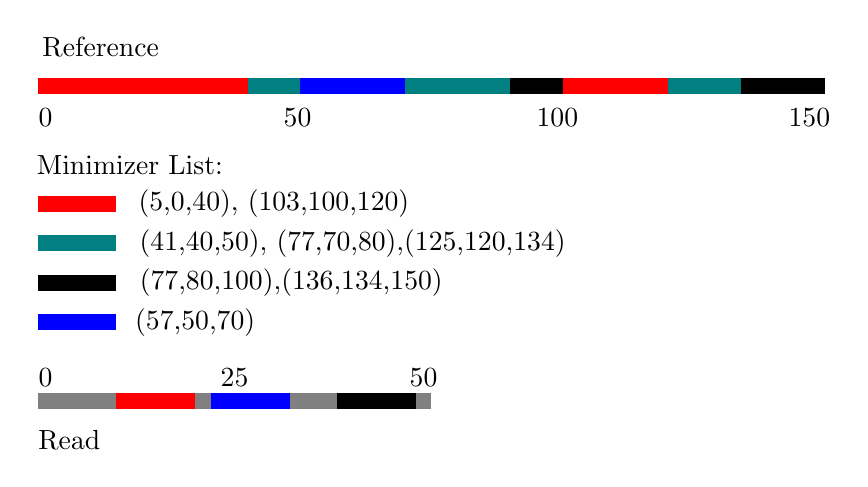
\begin{tikzpicture}[]
		
		%reference
		\draw[line width=2mm] (0,4) -- (10,4);
		\draw[line width=2mm,color=red] (0,4) -- (2.67,4);
		\draw[line width=2mm,color=green!50!blue] (2.67,4) -- (5,4);
		\draw[line width=2mm,color=blue] (3.33,4) -- (4.67,4);
		\draw[line width=2mm,color=green!50!blue] (4.67,4) -- (6,4);
		\draw[line width=2mm,color=red] (6.67,4) -- (8,4);
		\draw[line width=2mm,color=green!50!blue] (8,4) -- (8.93,4);
		%read
		\draw[line width=2mm,color=black!50] (0,0) -- (5,0);
		\draw[line width=2mm,color=red] (1,0) -- (2,0);
		\draw[line width=2mm,color=blue] (2.2,0) -- (3.2,0);
		\draw[line width=2mm,color=black] (3.8,0) -- (4.8,0);
		
		%others
		\draw[line width=2mm,color=red] (0,2.5) -- (1,2.5);
		\node[rectangle](refer) at (3,2.5) {(5,0,40), (103,100,120)};
		\draw[line width=2mm,color=green!50!blue] (0,2) -- (1,2);
		\node[rectangle](refer) at (4,2) {(41,40,50), (77,70,80),(125,120,134)};
		\draw[line width=2mm,color=black] (0,1.5) -- (1,1.5);
		\node[rectangle](refer) at (3.22,1.5) { (77,80,100),(136,134,150)};
		\draw[line width=2mm,color=blue] (0,1) -- (1,1);
		\node[rectangle](refer) at (2,1) { (57,50,70)};
		%labels
		\node[rectangle](refer) at (0.8,4.5) {Reference};
		\node[rectangle](refer) at (0.1,3.6) {0};
		\node[rectangle](refer) at (3.3,3.6) {50};
		\node[rectangle](refer) at (6.6,3.6) {100};
		\node[rectangle](refer) at (9.8,3.6) {150};
		\node[rectangle](refer) at (0.4,-0.5) {Read};
		\node[rectangle](refer) at (0.1,0.3) {0};
		\node[rectangle](refer) at (2.5,0.3) {25};
		\node[rectangle](refer) at (4.9,0.3) {50};
		\node[rectangle](refer) at (1.17,3) {Minimizer List:};
		%arrows
		%\draw[line width=1mm,color=black!50,->] (1.5,0.2) ..  controls (1.5,3.8) and (2.5,0.2) .. (2.5,3.8);
		%\draw[line width=1mm,color=black!50,->] (3.2,0.2) .. controls(3.2,3.8) and (8,0.2) .. (8,3.8);
		\end{tikzpicture}
		\caption{Mapping Minimizers.}
	\end{figure}
\end{frame}

\begin{frame}
	\frametitle{Minimizer Approach : Result}
	\begin{table}[]
		\centering
		\caption{Minimizer Hits For Increasing Error Rate.}
		\label{my-label}
		\begin{tabular}{|r|r|r|r|}
			\hline
			\multicolumn{1}{|c|}{\textbf{\begin{tabular}[c]{@{}c@{}}Error\\ (\%)\end{tabular}}} & \multicolumn{1}{c|}{\textbf{\begin{tabular}[c]{@{}c@{}}Found In \\ Reference\\ (\%)\end{tabular}}} & \multicolumn{1}{c|}{\textbf{\begin{tabular}[c]{@{}c@{}}Found In\\ Range\\ (\%)\end{tabular}}} & \multicolumn{1}{c|}{\textbf{\begin{tabular}[c]{@{}c@{}}Found Both In \\ and Out of Range\\ (\%)\end{tabular}}} \\ \hline
			0 & 99.96 & 69.2 & 30.7 \\ \hline
			5 & 71.8 & 62.4 & 27.2 \\ \hline
			10 & 53.8 & 52.8 & 25.5 \\ \hline
			15 & 43.5 & 47.4 & 21.7 \\ \hline
			20 & 34.8 & 39.8 & 17.9 \\ \hline
			45 & \alert{0.2} & 40 & 40 \\ \hline
		\end{tabular}
	\end{table}
\end{frame}

\begin{frame}
	\frametitle{Gapped Minimizer}
	\begin{alertblock}{Problem}
		The More The Error, The More The Mismatches
	\end{alertblock}
	\pause
	{
		\setbeamercolor{block body}{bg=green!10,fg=black}
		\setbeamercolor{block title}{bg=green!50!black,fg=white}
	\begin{block}{Solution}
		Insert Gap in Both Reads and Reference To Neutralize Mismatches At Every Certain Number of Bases.
	\end{block}
	}	
	\pause
	\begin{block}{Remark}
		In NanoMapper, Gaps are Added Every Third Base Assuming 33\% Error.\\
		Example:  \texttt{ATCTGGTAATCATAGCGTAC}\\
		With Gap: \texttt{AT\_TG\_TA\_TC\_TA\_CG\_AC}
	\end{block}
\end{frame}